\famichapter{Core Feature Implementation}{This chapter explains the core features
of FamiPet using their workflows, data, validation, and security behaviour, each
supported by a diagram.}{ch:features}

\section{Digital Pet Identity and QR Code}

\begin{figure}[htbp]
    \centering
    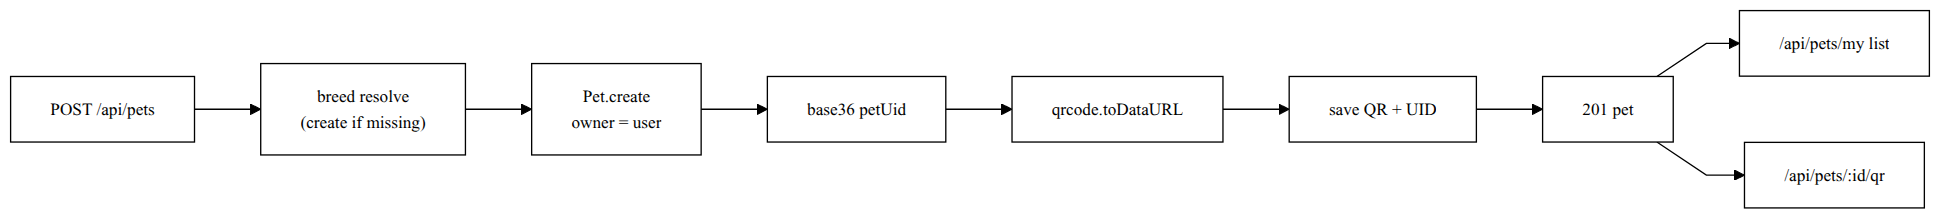
\includegraphics[width=\textwidth]{figures/13-pet-qr.png}
    \caption{Creation of a pet with automatic QR identity.}
    \label{fig:petqr}
\end{figure}

When a user creates a pet (\texttt{POST /api/pets}), the controller accepts
either a breed \texttt{ObjectId} or a breed name; a name is resolved to a breed
document and created on demand if absent. The pet is stored with
\texttt{owner: req.user.id}. A unique digital pet identifier is then generated
as \texttt{Date.now().toString(36)-petId.\allowbreak{}slice(-8)-random} and the
\texttt{qrcode} package encodes a JSON payload with the pet identifier, unique
ID, name, species, and breed into a PNG data URL that is persisted on the pet
document. The pet appears in the owner's list (\texttt{GET /api/pets/my}), and
the dedicated endpoint \texttt{GET /api/pets/:id/qr} regenerates a QR code whose
payload additionally includes the owner's public name and phone. The digital pet
identity is deliberately public-safe: the QR payload contains only identity and
public contact fields, never tokens, passwords, or the account reference
directly.

\section{Adoption Management}

\begin{figure}[htbp]
    \centering
    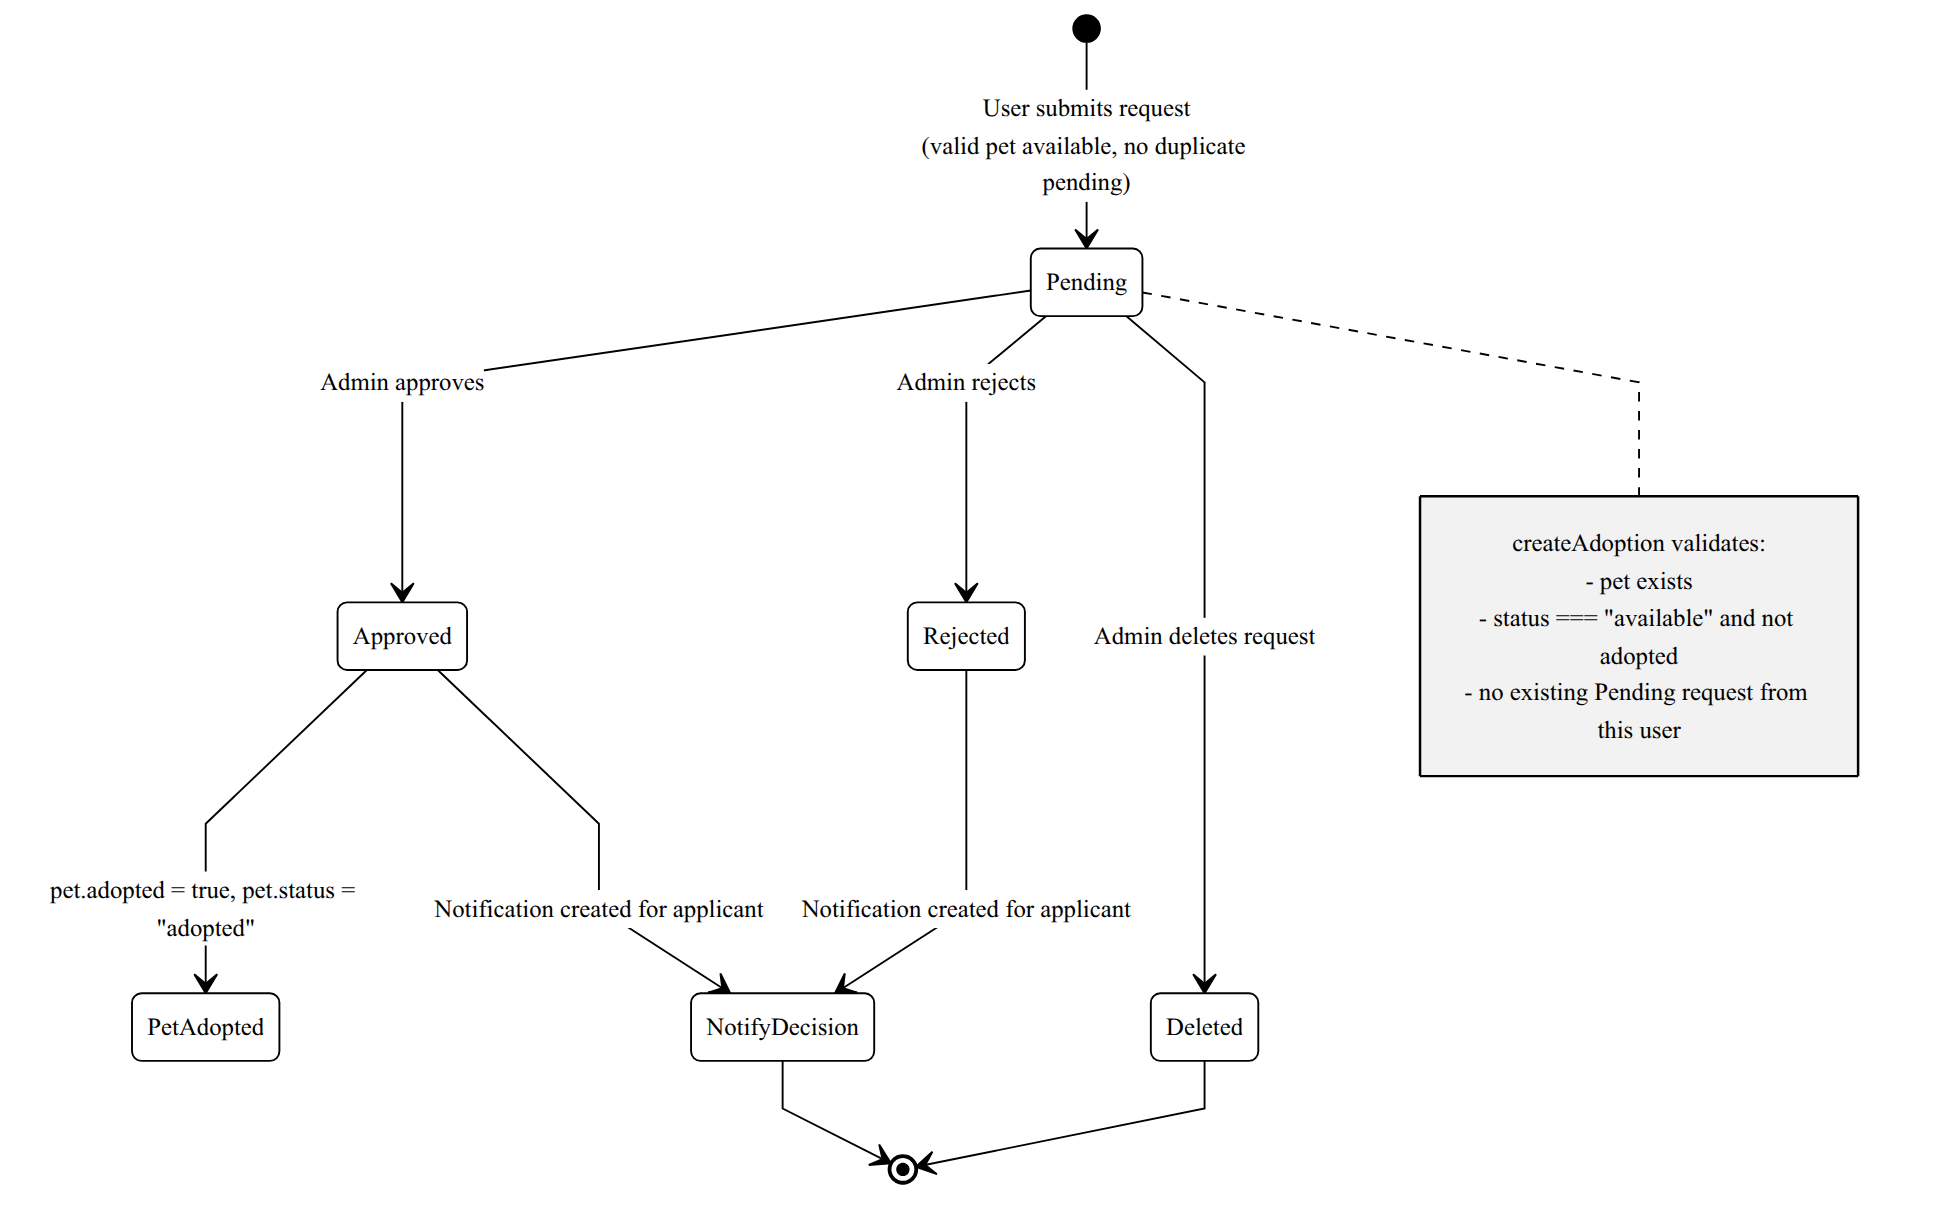
\includegraphics[width=\textwidth]{figures/14-adoption-state.png}
    \caption{Adoption request state diagram.}
    \label{fig:adoptstate}
\end{figure}

An adoption request (\texttt{POST /api/adoptions}) requires the pet reference,
full name, phone, address, and a reason. The controller verifies that the pet
exists, is \texttt{status: "available"} and not \texttt{adopted}, and that the
user has no already-pending request for the same pet; a duplicate is rejected.
The request is stored in the \texttt{Pending} state. Administrators transition
the state to \texttt{Approved} or \texttt{Rejected} through
\texttt{PUT /api/adoptions/:id} (admin-only). Approval automatically updates the
pet document (\texttt{adopted: true}, \texttt{status: "adopted"}), and every
status change creates a notification for the applicant with the pet's name and
the new state.

\begin{figure}[htbp]
    \centering
    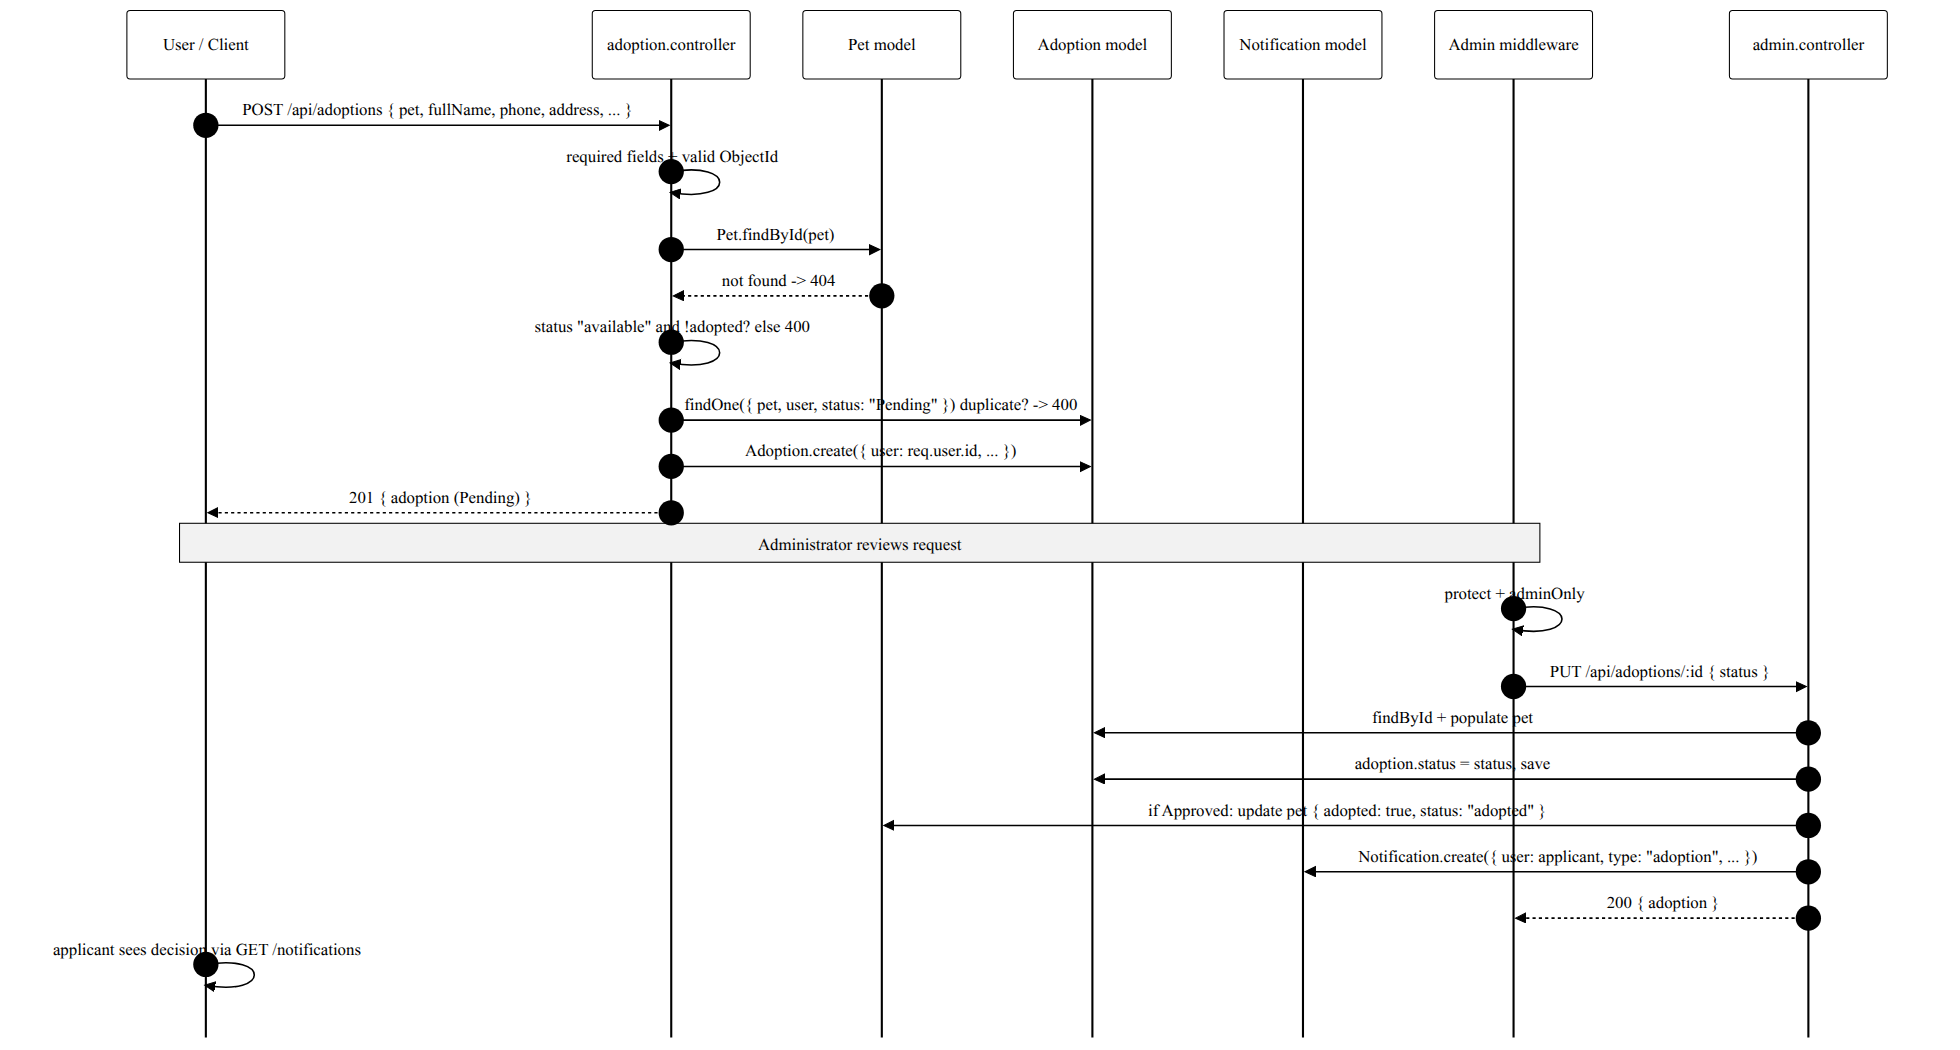
\includegraphics[width=\textwidth]{figures/15-adoption-sequence.png}
    \caption{Adoption application and approval sequence.}
    \label{fig:adoptseq}
\end{figure}

The sequence diagram shows the full path: the user submits the application, the
owners own pet records feed the adoption listing, the administrator reviews and
approves the request, the backend updates the pet and creates the applicant
notification, and the applicant reads both the updated request state and the
notification. Notification and pet-record data are stored in MongoDB, so both
survive a page reload.

\section{Appointments, Notifications, and Reminders}

Booking an appointment (\texttt{POST /api/appointments}) validates the pet and
veterinarian references, requires the pet to belong to the requesting user and
the veterinarian to be active, and rejects a double booking: an existing
appointment with the same veterinarian, date, and time in the
\texttt{pending} or \texttt{confirmed} state returns HTTP 400.

\begin{figure}[htbp]
    \centering
    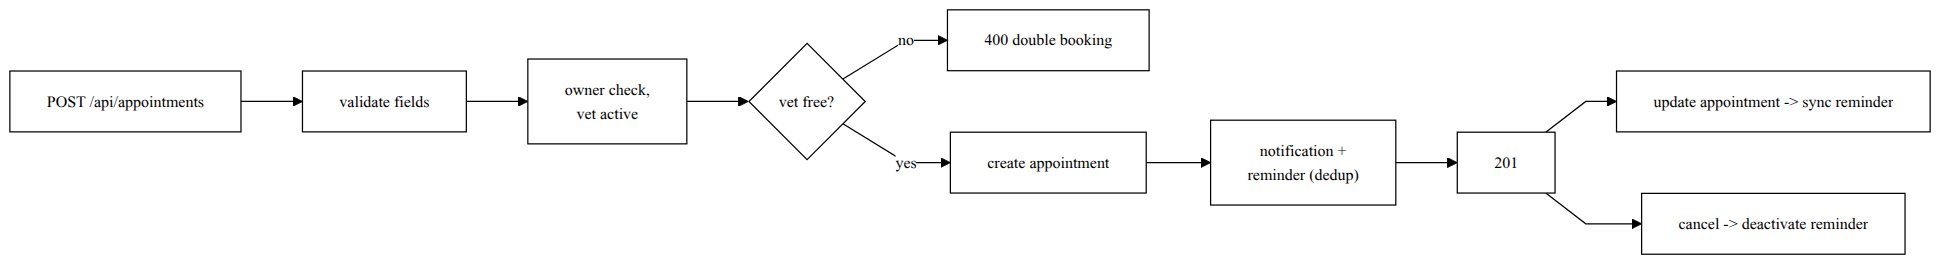
\includegraphics[width=\textwidth]{figures/16-appointment-flow.png}
    \caption{Appointment booking, rescheduling, and cancellation flow.}
    \label{fig:apptflow}
\end{figure}

On success the controller creates the appointment, immediately creates a
\texttt{Notification} (type \texttt{appointment}), and creates a
\texttt{Reminder} (type \texttt{appointment}, frequency \texttt{once}), but only
if an identical active reminder does not already exist, so repeat bookings do
not duplicate reminders. Rescheduling an appointment synchronizes the date and
time of the matching reminder; cancelling sets the appointment to
\texttt{cancelled} and deactivates the matching reminder so no stale active
reminder remains.

\begin{figure}[htbp]
    \centering
    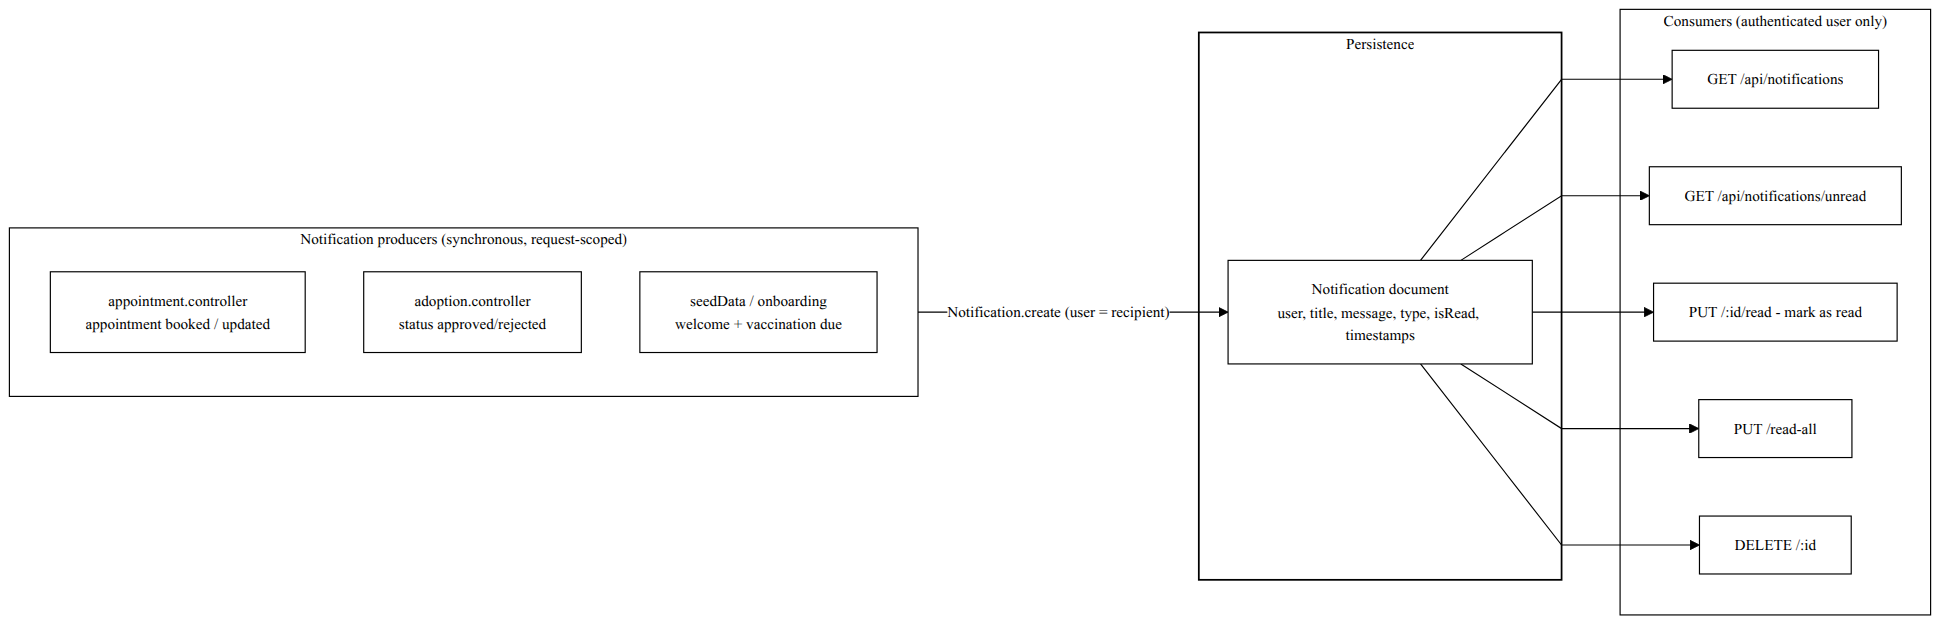
\includegraphics[width=\textwidth]{figures/17-notification-flow.png}
    \caption{Notification creation and consumption flow.}
    \label{fig:notifflow}
\end{figure}

Notifications are the shared feedback channel of the platform. They are created
by the adoption and appointment controllers and read through the notification
API, which is scoped to the owner and supports an unread filter, mark-as-read,
mark-all-as-read, and deletion. The read state persists, so notifications remain
correctly unread/read across reloads.

\begin{figure}[htbp]
    \centering
    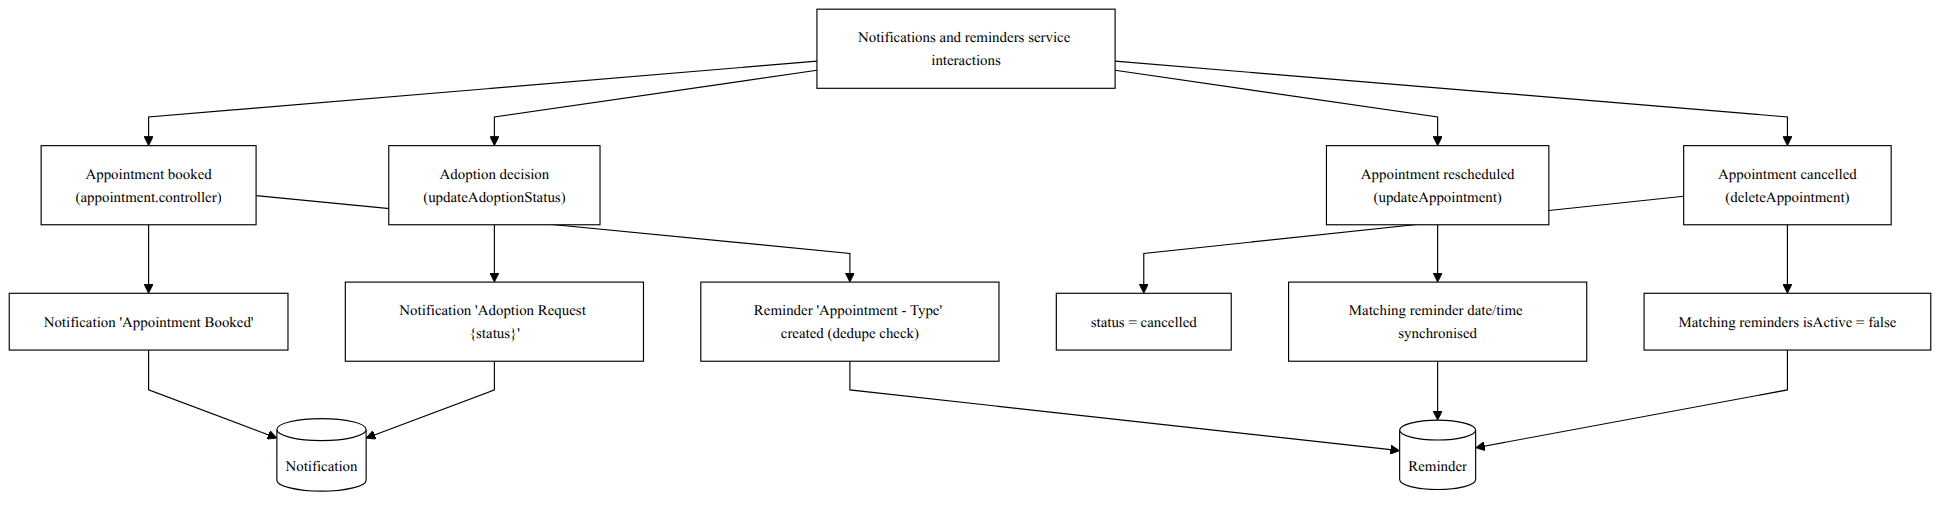
\includegraphics[width=\textwidth]{figures/20-notif-reminder-sync.png}
    \caption{Synchronization between appointments, notifications, and reminders.}
    \label{fig:notifrem}
\end{figure}

The synchronization diagram is a summary of the invariant demonstrated by the
implementation: booking creates the notification and reminder; rescheduling
moves the reminder; cancellation flips the appointment state and deactivates the
reminder. No background job is involved; all effects are applied synchronously
in the request handler against the same MongoDB store.

\section{PetGPT -- the AI Assistant}

\begin{figure}[htbp]
    \centering
    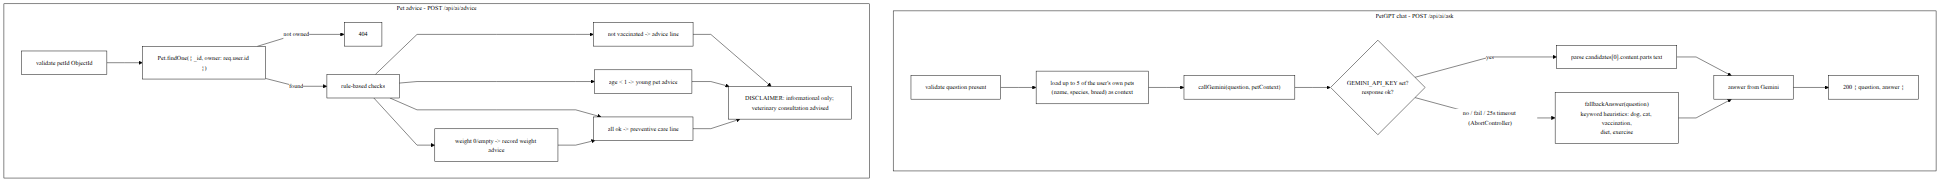
\includegraphics[width=\textwidth]{figures/18-ai-pipeline.png}
    \caption{PetGPT request pipeline with fallback.}
    \label{fig:aipipe}
\end{figure}

The AI subsystem exposes two endpoints. \texttt{POST /api/ai/ask} takes a
question, loads up to five of the user's own pets (name, species, breed) as
context, and calls the Google Gemini REST endpoint
(\texttt{gemini-1.5-flash}) with a PetGPT system instruction and a 25-second
timeout through an \texttt{AbortController}. If the API key is missing, the
call fails, or times out, a built-in keyword fallback returns safe generic
guidance for common topics (dogs, cats, vaccination, diet, exercise). The
second endpoint, \texttt{POST /api/ai/advice}, is fully rule-based: it requires
a pet owned by the user and produces advice from the pet's actual
\texttt{vaccinated} flag, age, and weight, recommending professional veterinary
care when a vaccination or weight record is missing. The assistant therefore
never fabricates a diagnosis; its output is either model-generated general
advice or profile-derived advice from real records.

\section{Community and Lost-and-Found}

\texttt{POST /api/community} creates a post (optionally with an image) bound to
the authenticated user. Likes and comments are embedded arrays; like toggling
adds or removes the user reference, so re-pressing a like cancels it. Posts are
listed publicly, but only when \texttt{isActive: true}. Post, comment, and
lost-and-found report deletion allow either the owner or an administrator.
Lost-and-found reports carry type (\texttt{lost}/\texttt{found}), pet
attributes, location, date, and contact details, with an
\texttt{active}/\texttt{resolved} status that administrators can update.
Ownership checks are identical in shape to the other subsystems: the report is
queried with the owner predicate and the controller verifies
\texttt{report.user} against \texttt{req.user.id} before modification.

\section{Feature Verification Summary}

Each feature described in this chapter was exercised end-to-end in the test
campaign of Chapter~\ref{ch:testing}: pets and QR, favourites, adoption through
to admin approval, appointments with automatic notification and reminder
creation, cancellation deactivating the reminder, community posts with images,
likes and comments, lost-and-found reporting, health records, vaccinations, and
notifications. The persistence, read-back, and cleanup behaviour of every
feature was verified against MongoDB.